%%%%%%%%%%%%%%%%%%%%%%%%%%%%%%%%%%%%%%%%%%%%%%%%%%%%%%%%%%%%%%%%%%%%%%%%%%%
%
% Plantilla para un artículo en LaTeX en español.
%
%%%%%%%%%%%%%%%%%%%%%%%%%%%%%%%%%%%%%%%%%%%%%%%%%%%%%%%%%%%%%%%%%%%%%%%%%%%



%--------------------------------------------------------------------------
\title{Plantilla para un artículo \LaTeX}
\author{El autor va aquí\\
  \small Dept. Plantillas y Editores\\
  \small E12345\\
  \small España
}

\begin{document}
\section{PRACTICA DE LABORATORIO N° 01:}
\item{
Elaboración de Dashboards en Power BI


\section{REQUERIMIENTOS}
\item{Conocimientos
Para el desarrollo de esta práctica se requerirá de los siguientes conocimientos básicos:\\
- Conocimientos básicos de administración de base de datos Microsoft SQL Server.\\
- Conocimientos básicos de SQL.\\
✓ Software
Asimismo se necesita los siguientes aplicativos:
- Microsoft SQL Server 2016 o superior\\
- Base de datos AdventureWorks2016 o superior\\
- Power BI Desktop.\\
- Tener una cuenta Microsoft registrada en el Portal de Power Bi}\\

\section{CONSIDERACIONES INICIALES}
\item{Generar una carpeta o directorio Power BI en un lugar accesible para guardar los resultados de la práctica.}
\section{DESARROLLO}
\item{Cuando la Ventana de Power BI Desktop aparezca, en el panel a mano izquierda, hacer click en Obtener
Datos (Get Data).}
\begin{figure}[httb]
\begin{center}
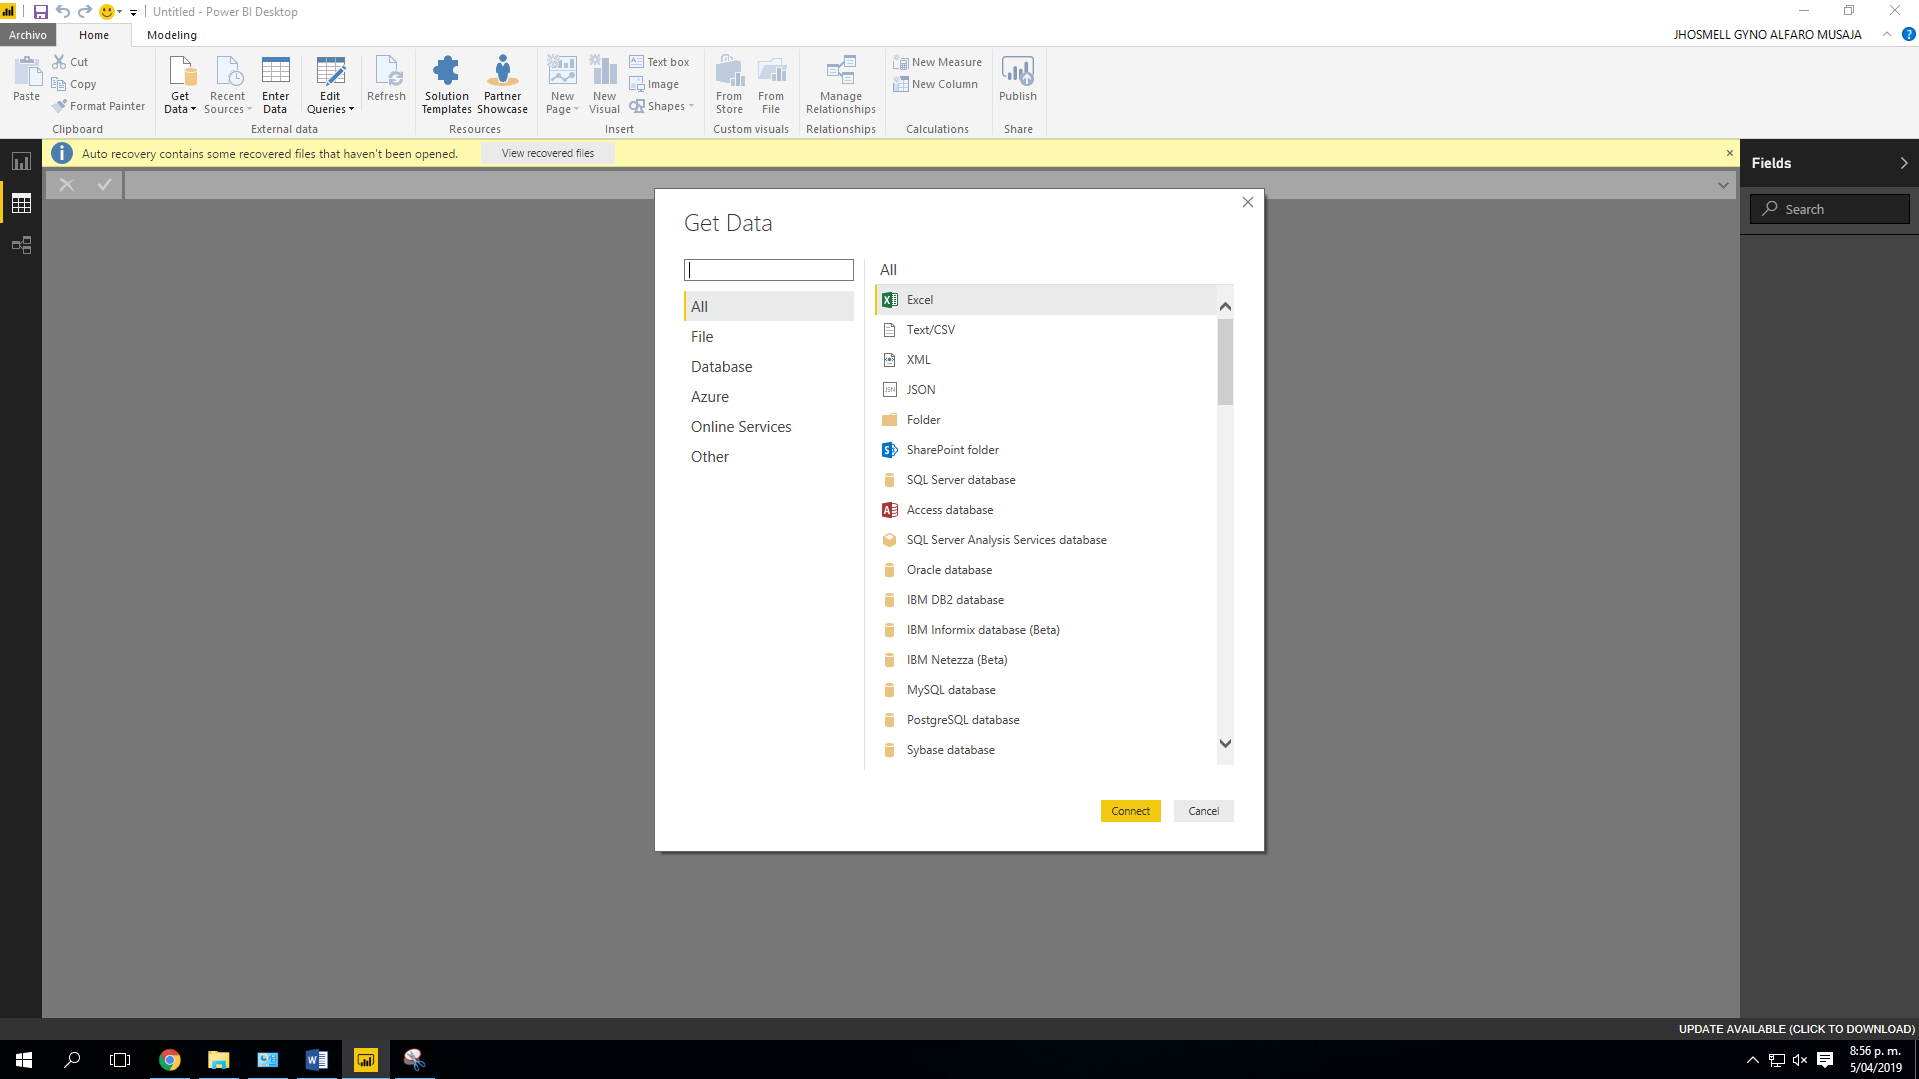
\includegraphics[width=15cm]{./Imagenes/image001}
\end{center}
\end{figure}
\item{ En el cuadro de dialogo Obtener Datos (Get Data), click en base de datos SQL Server, y luego hacer click en
Conectar (Connect). }
\begin{figure}[httb]
\begin{center}
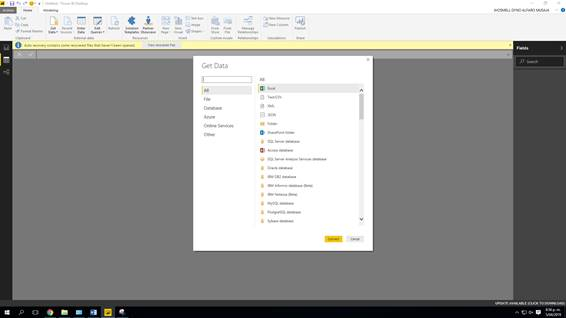
\includegraphics[width=15cm]{./Imagenes/image002}
\end{center}
\end{figure}

\item{  En el cuadro de dialogo base de datos SQL Server, en la casilla servidor tipear (local), en la casilla Base de
datos (opcional) / Database (optional), tipear AdventureWorks2017, y hacer clic en OK. }
\begin{figure}[httb]
\begin{center}
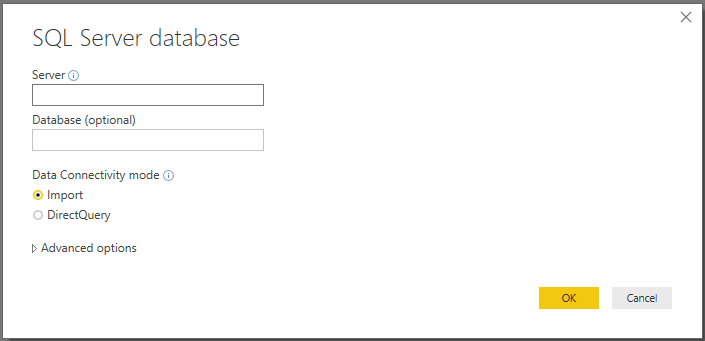
\includegraphics[width=15cm]{./Imagenes/image003}
\end{center}
\end{figure}
\newpage
\item{ En el menu principal (Home ribbon), hacer click en Funetes Recientes (Recent Sources), y en local:
AdventureWorks2017. }
\begin{figure}[httb]
\begin{center}
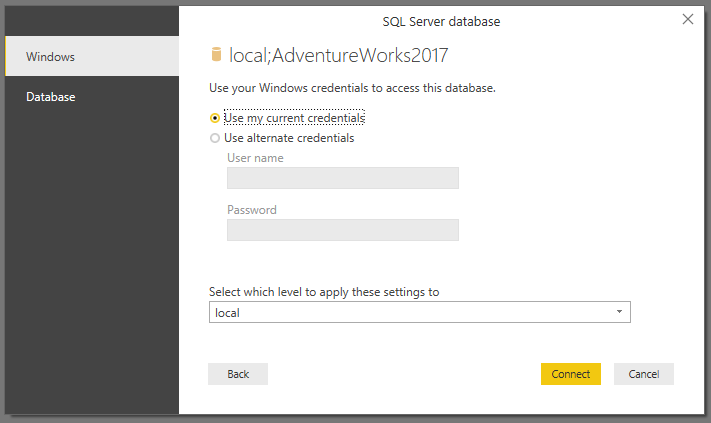
\includegraphics[width=10cm]{./Imagenes/image005}
\end{center}
\end{figure}
\item{ Agregamos datos para trabajar las figuras. }
\begin{figure}[httb]
\begin{center}
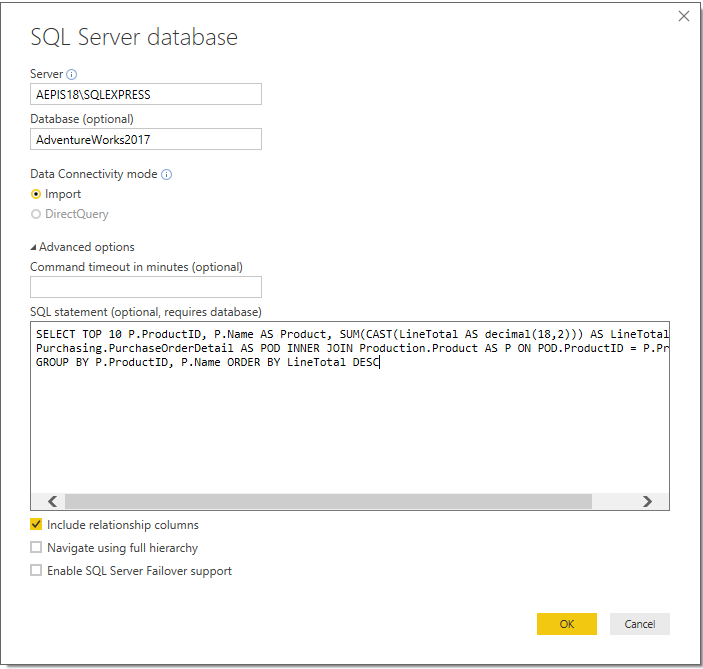
\includegraphics[width=10cm]{./Imagenes/image015}
\end{center}
\end{figure}
\newpage
\item{ Al tendremos las siguientes graficos con los datos obtenidos de la base de datos AdventureWorks2017. }
\begin{figure}[httb]
\begin{center}
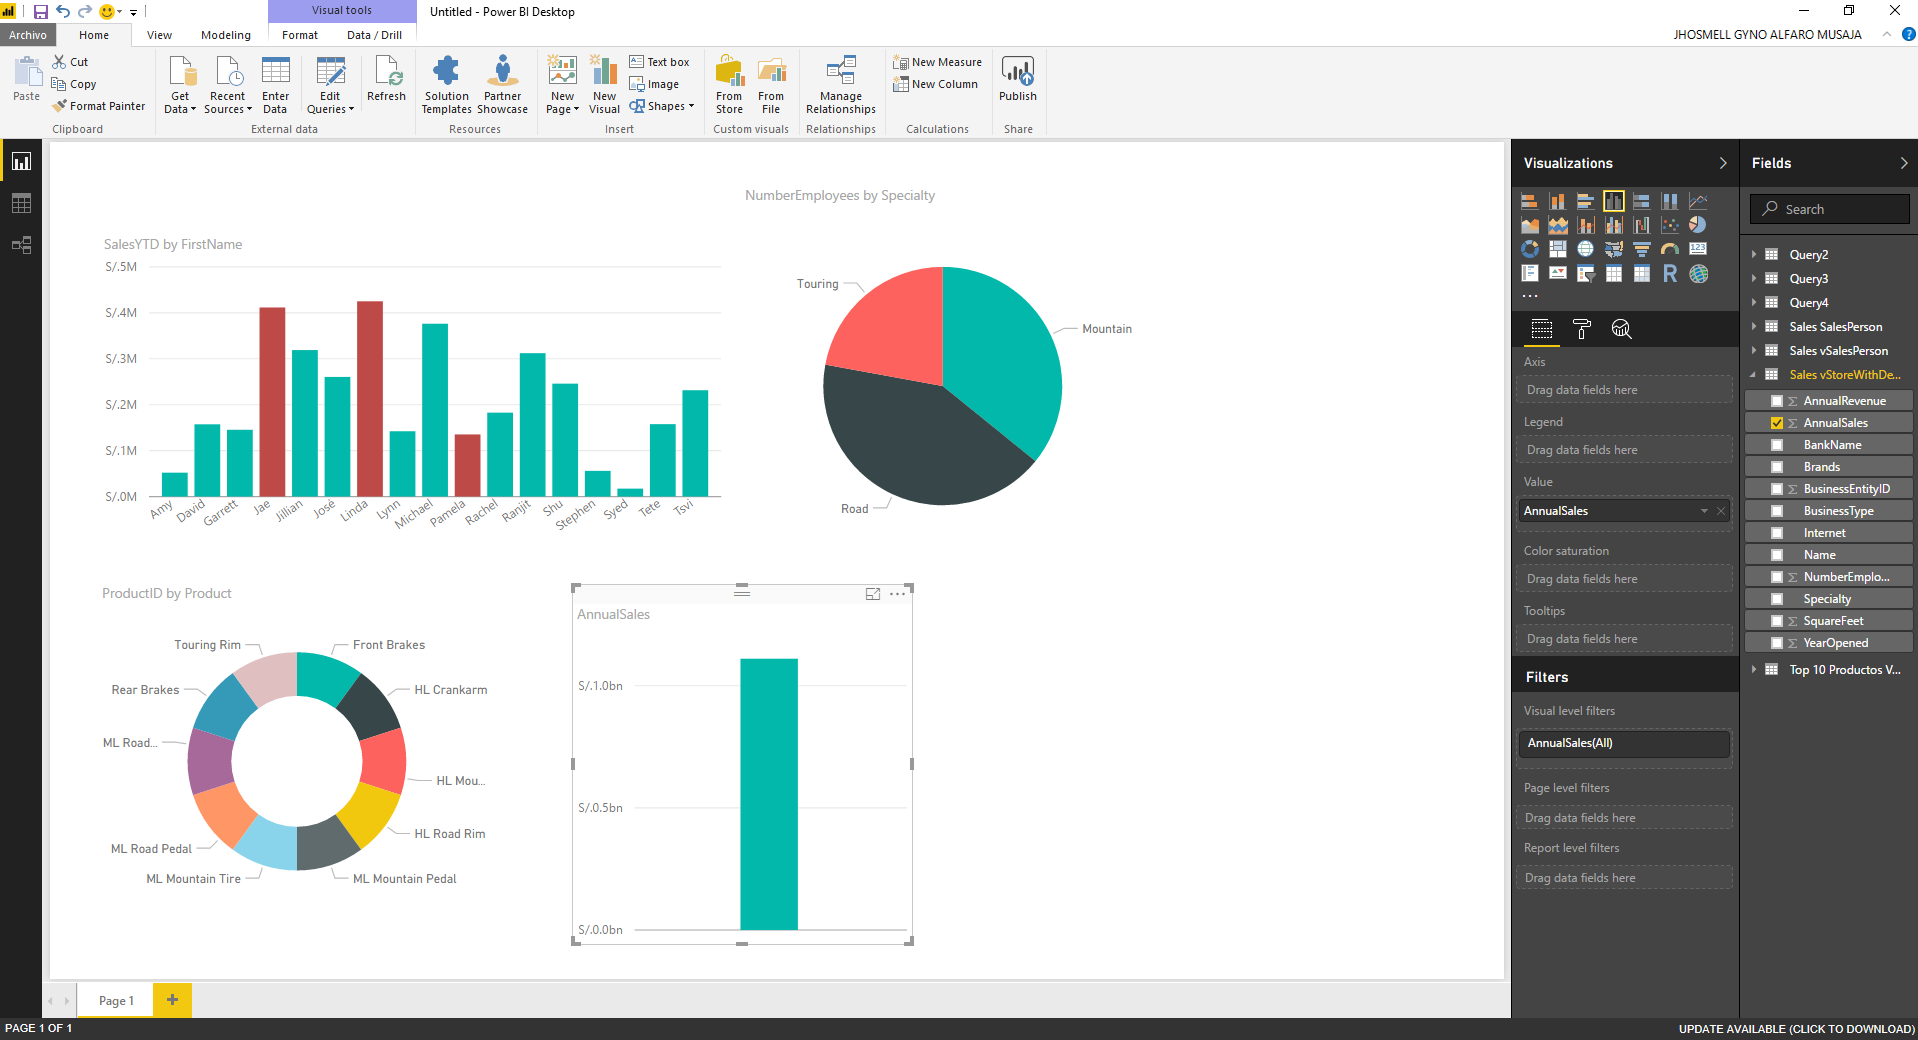
\includegraphics[width=15cm]{./Imagenes/image034}
\end{center}
\end{figure}
\item{Guardamos y Subimos nuestro proyecto a nuestra cuenta de powerbi . }
\begin{figure}[httb]
\begin{center}
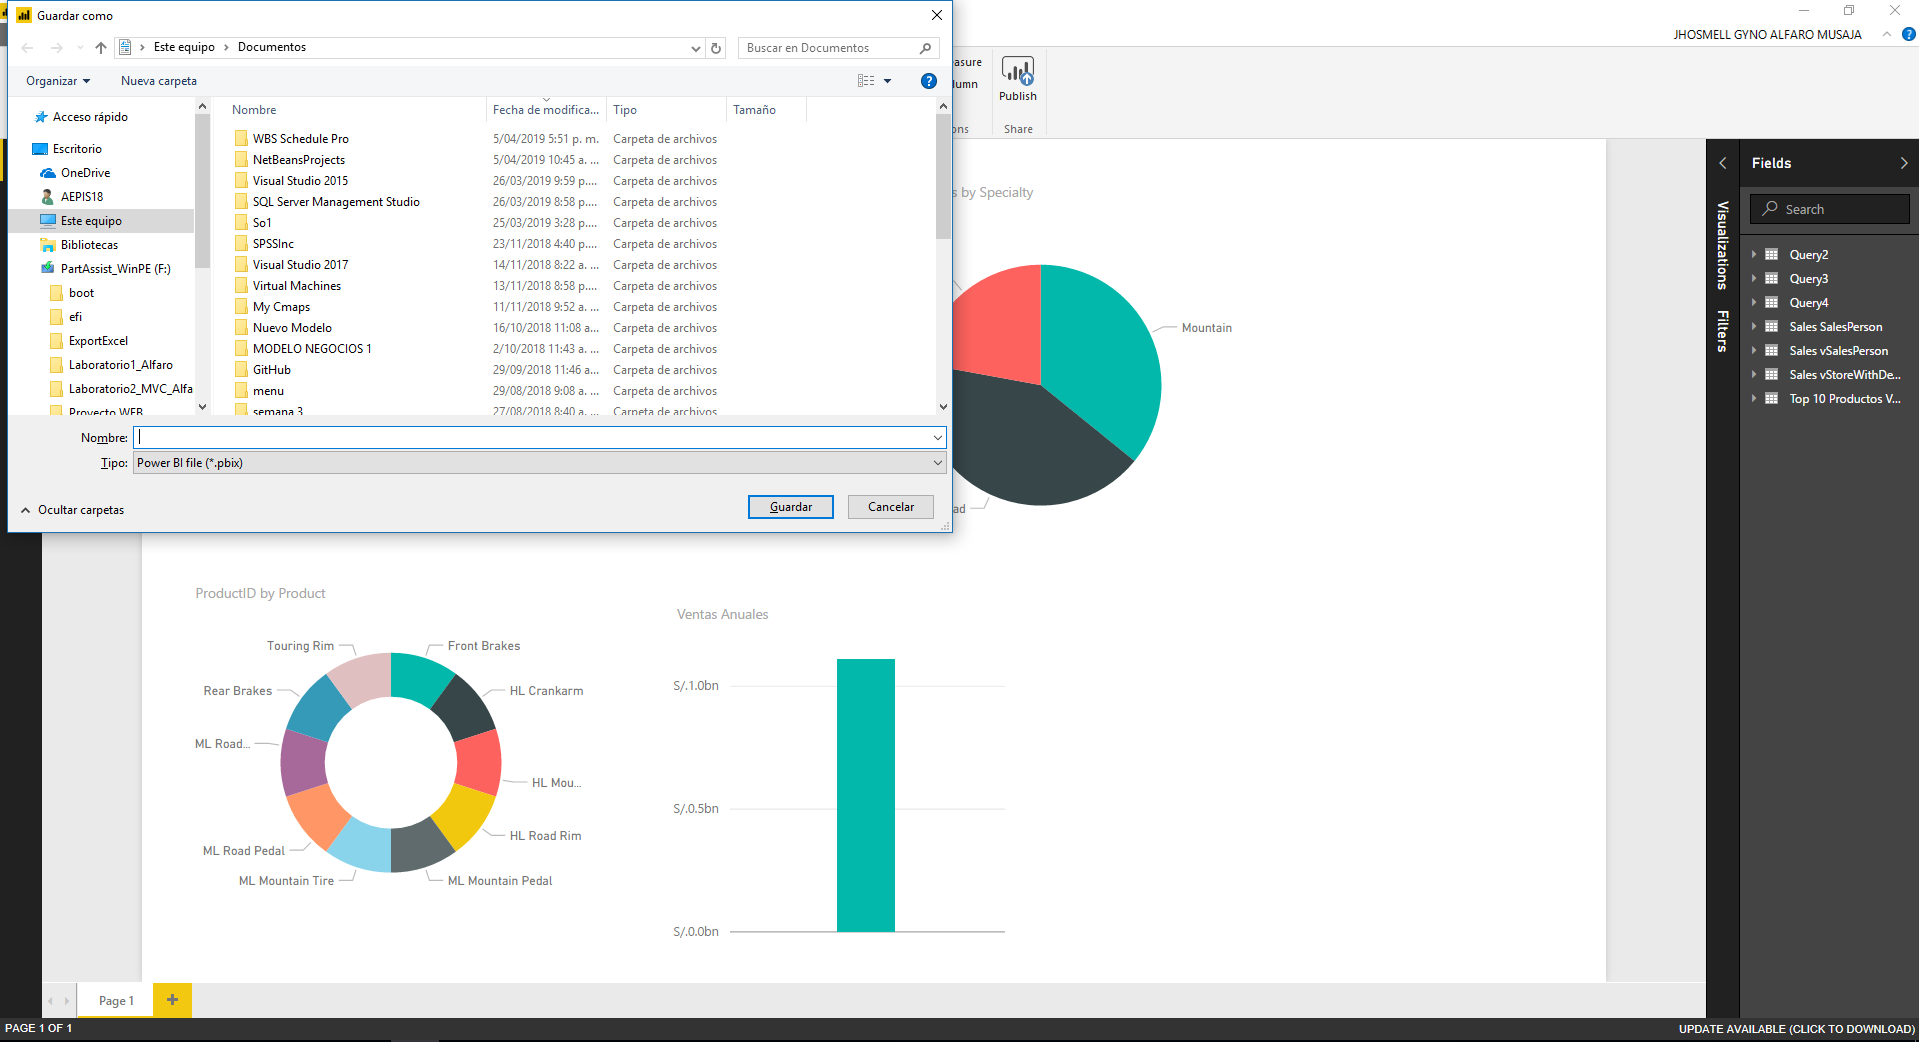
\includegraphics[width=15cm]{./Imagenes/image038}
\end{center}
\end{figure}

\item{el link para poder vizulaizar el trabajo encargado numero 1 .\\
https://app.powerbi.com/groups/me/reports/8e58d7bc-0331-4ad6-b99c-7ff974e859ce?ctid=b6b466ee-468d-4011-b9fc-fbdcf82ac90a}



\end{document}
